\documentclass[10pt]{beamer}\usepackage[]{graphicx}\usepackage[]{color}
%% maxwidth is the original width if it is less than linewidth
%% otherwise use linewidth (to make sure the graphics do not exceed the margin)
\makeatletter
\def\maxwidth{ %
  \ifdim\Gin@nat@width>\linewidth
    \linewidth
  \else
    \Gin@nat@width
  \fi
}
\makeatother

\definecolor{fgcolor}{rgb}{0.345, 0.345, 0.345}
\newcommand{\hlnum}[1]{\textcolor[rgb]{0.686,0.059,0.569}{#1}}%
\newcommand{\hlstr}[1]{\textcolor[rgb]{0.192,0.494,0.8}{#1}}%
\newcommand{\hlcom}[1]{\textcolor[rgb]{0.678,0.584,0.686}{\textit{#1}}}%
\newcommand{\hlopt}[1]{\textcolor[rgb]{0,0,0}{#1}}%
\newcommand{\hlstd}[1]{\textcolor[rgb]{0.345,0.345,0.345}{#1}}%
\newcommand{\hlkwa}[1]{\textcolor[rgb]{0.161,0.373,0.58}{\textbf{#1}}}%
\newcommand{\hlkwb}[1]{\textcolor[rgb]{0.69,0.353,0.396}{#1}}%
\newcommand{\hlkwc}[1]{\textcolor[rgb]{0.333,0.667,0.333}{#1}}%
\newcommand{\hlkwd}[1]{\textcolor[rgb]{0.737,0.353,0.396}{\textbf{#1}}}%

\usepackage{framed}
\makeatletter
\newenvironment{kframe}{%
 \def\at@end@of@kframe{}%
 \ifinner\ifhmode%
  \def\at@end@of@kframe{\end{minipage}}%
  \begin{minipage}{\columnwidth}%
 \fi\fi%
 \def\FrameCommand##1{\hskip\@totalleftmargin \hskip-\fboxsep
 \colorbox{shadecolor}{##1}\hskip-\fboxsep
     % There is no \\@totalrightmargin, so:
     \hskip-\linewidth \hskip-\@totalleftmargin \hskip\columnwidth}%
 \MakeFramed {\advance\hsize-\width
   \@totalleftmargin\z@ \linewidth\hsize
   \@setminipage}}%
 {\par\unskip\endMakeFramed%
 \at@end@of@kframe}
\makeatother

\definecolor{shadecolor}{rgb}{.97, .97, .97}
\definecolor{messagecolor}{rgb}{0, 0, 0}
\definecolor{warningcolor}{rgb}{1, 0, 1}
\definecolor{errorcolor}{rgb}{1, 0, 0}
\newenvironment{knitrout}{}{} % an empty environment to be redefined in TeX

\usepackage{alltt}
\usepackage[utf8]{inputenc}

	\usetheme{Warsaw}


\usepackage{amsmath}						% paquete para expresiones matemáticas
\usepackage{amsfonts}					% paquete para escritura de ecuaciones 
\usepackage{amssymb}						% paquete para caracteres especiales para ecuaciones 

\usepackage{fancyhdr}					% Temas para encabezado y pie de pagina
\usepackage{fancyvrb}
\pagestyle{fancy} 

\pagenumbering{arabic} 					% Numeración de paginas {arabic roman}
\usepackage{hyperref}					% Para hipervinculos
\usepackage{graphicx}					% Para incluir imágenes
\usepackage{ float}
\usepackage{caption}						% Descripciones de las figuras
\usepackage{subcaption}					% Descripción varias imagenes en usa sola figura
\graphicspath{ {Imagenes/} }				% Directorio de imágenes esta capeta va donde esta el archivo tex


\usepackage{color, colortbl}				% Colores para tablas
\usepackage{listings}					% Para el código Fuente
\usepackage{xcolor}						% para color en codigos o listrings
\definecolor{limegreen}{RGB}{50,100,50}	% Definición de colores ejemplo verde en RGB
\definecolor{Red}{RGB}{220,120,120}		% se definen colores para la tabla en el cronograma 
\definecolor{LightCyan}{rgb}{0.88,1,1}
\definecolor{azul}{RGB}{120,120,210}

%para pytohn
\DeclareFixedFont{\ttb}{T1}{txtt}{bx}{n}{9} % for bold
\DeclareFixedFont{\ttm}{T1}{txtt}{m}{n}{9}  % for normal
\definecolor{deepblue}{rgb}{0,0,0.5}
\definecolor{deepred}{rgb}{0.6,0,0}
\definecolor{deepgreen}{rgb}{0,0.5,0}

\newcommand\pythonstyle{\lstset{
		language=Python,
		basicstyle=\ttm,
		otherkeywords={self},             % Add keywords here
		keywordstyle=\ttb\color{deepblue},
		emph={MyClass,__init__},          % Custom highlighting
		emphstyle=\ttb\color{deepred},    % Custom highlighting style
		stringstyle=\color{deepgreen},
		frame=tb,                         % Any extra options here
		showstringspaces=false            % 
	}}
	
	
	% Python environment
	\lstnewenvironment{python}[1][]
	{
		\pythonstyle
		\lstset{#1}
	}
	{}
	
	% Python for external files
	\newcommand\pythonexternal[2][]{{
			\pythonstyle
			\lstinputlisting[#1]{#2}}}
	
	% Python for inline
	\newcommand\pythoninline[1]{{\pythonstyle\lstinline!#1!}}
	
	
	%%%%
	\lstdefinestyle{base}{
		language=C,
		emptylines=1,
		breaklines=true,
		showspaces=fasle,
		showstringspaces=false,
		extendedchars=true,
		basicstyle=\ttfamily\color{black},
		moredelim=**[is][\color{limegreen}]{'}{'}, 	% Para este caso especial el caracter ' y & encierran
		moredelim=**[is][\color{blue}]{&}{&},		% un fragmento de código que quiere ser coloreado
	}
	
	\lstset{numbers=left, numberstyle=\tiny, stepnumber=2, numbersep=5pt}
	
	\definecolor{dkgreen}{rgb}{0,0.6,0}
	\definecolor{gray}{rgb}{0.5,0.5,0.5}
	\definecolor{mauve}{rgb}{0.58,0,0.82}
	
	\lstset{frame=tb,
		language=R,
		aboveskip=3mm,
		belowskip=3mm,
		showstringspaces=false,
		columns=flexible,
		numbers=none,
		keywordstyle=\color{blue},
		numberstyle=\tiny\color{gray},
		commentstyle=\color{dkgreen},
		stringstyle=\color{mauve},
		breaklines=true,
		breakatwhitespace=true,
		tabsize=3
	}
\IfFileExists{upquote.sty}{\usepackage{upquote}}{}
\begin{document}


\title[Referencias Cruzadas]{Sistema para adquisición de datos para el control y supervisión de cultivos domésticos por protocolo IPV6}
		%Logo Gráfica Escudo Universidad Vectorizado.
		\logo{
\includegraphics[scale=0.08]{escudoud}}
		%Autor, Universidad, Fecha..
		\author{Wilson Ricardo López Sánchez }
		\institute[UD]{Universidad Distrital Francisco Jose de Caldas}
		\date{\today}


\begin{frame}
	       	%Titulo de la pagina
			\titlepage 
		\end{frame}
		
\begin{frame}
\frametitle{Introducción}
    Techos verdes
	\begin{figure}[ht] % Es preferible verificar la documentación para que la imagen quede correctamente segun el parámetro entre []
		\centering
		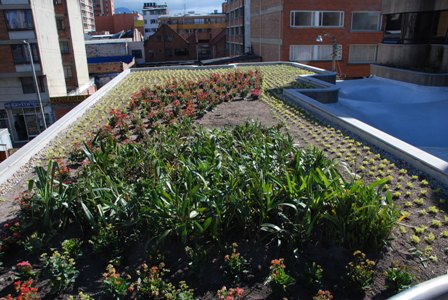
\includegraphics[scale=2]{techoverde}   % Scale se utiliza para cambiar el tamaño de la imagen
		\caption{Terraza piso 3 Secretaria Distrital de Ambiente}
		
	\end{figure}
\end{frame}

\begin{frame}
\frametitle{Descripción del proyecto}
	\begin{itemize}
		\item \textbf{Adquisición de datos:} Los datos se simularan 
		\item \textbf{Actuadores:} control un actuador desde la raspberry y una pagina html		
		\item \textbf{Comunicación IPv6:} Comunicación IPv6 se trabajara en la red interna de la universidad 
		\item\textbf{ Visualización de los datos en la nube:} Ubidots 
			
	\end{itemize}
\end{frame}

\begin{frame}
\frametitle{Objetivos}
\textbf{General}
	\begin{itemize}
		\item Diseñar y realizar un prototipo de un sistema para adquisición de datos para el control y supervisión de cultivos domésticos por protocolo IPV6
	\end{itemize}
	
\textbf{Especificos}
	\begin{itemize}
		\item diseñar un dispositivo para la adquisición y control de variables (temperatura y humedad)
		\item diseñar he implementar comunicación por IPv6 entre los dispositivos.
		\item Implementar sistema para visualizar los datos adquiridos en la nube 
	\end{itemize}
\end{frame}

\begin{frame}
\frametitle{Desarrollo del proyecto}

{\Huge Desarrollo del proyecto}

\end{frame}

\begin{frame}
\frametitle{Preparación de la Raspberry}
\begin{itemize}
	\item Instalar S.O.
	\item instalar paquetes
			
			\begin{small}
		\vspace{sudo apt-get update\\				
				sudo apt-get upgrade\\
				sudo apt-get install python\\
				sudo apt-get install python-dev\\
				sudo apt-get install libjpeg-dev\\
				sudo apt-get install libfreetype6-dev\\
				sudo apt-get install python-setuptools\\
				sudo apt-get install python-rpi.gpio\\
				sudo easy\_install pip\\
				sudo pip install ubidots\\
				sudo apt-get install python-pip\\
				pip install tornado\\
				pip install --upgrade pip }					
				
			\end{small}		
\end{itemize}

\end{frame}



\begin{frame}
\frametitle{Ubidots}
Ubidots es un servicio en la nube que permite almacenar y analizar información de sensores en tiempo real:
 	\begin{figure}[ht]
 		\centering
 		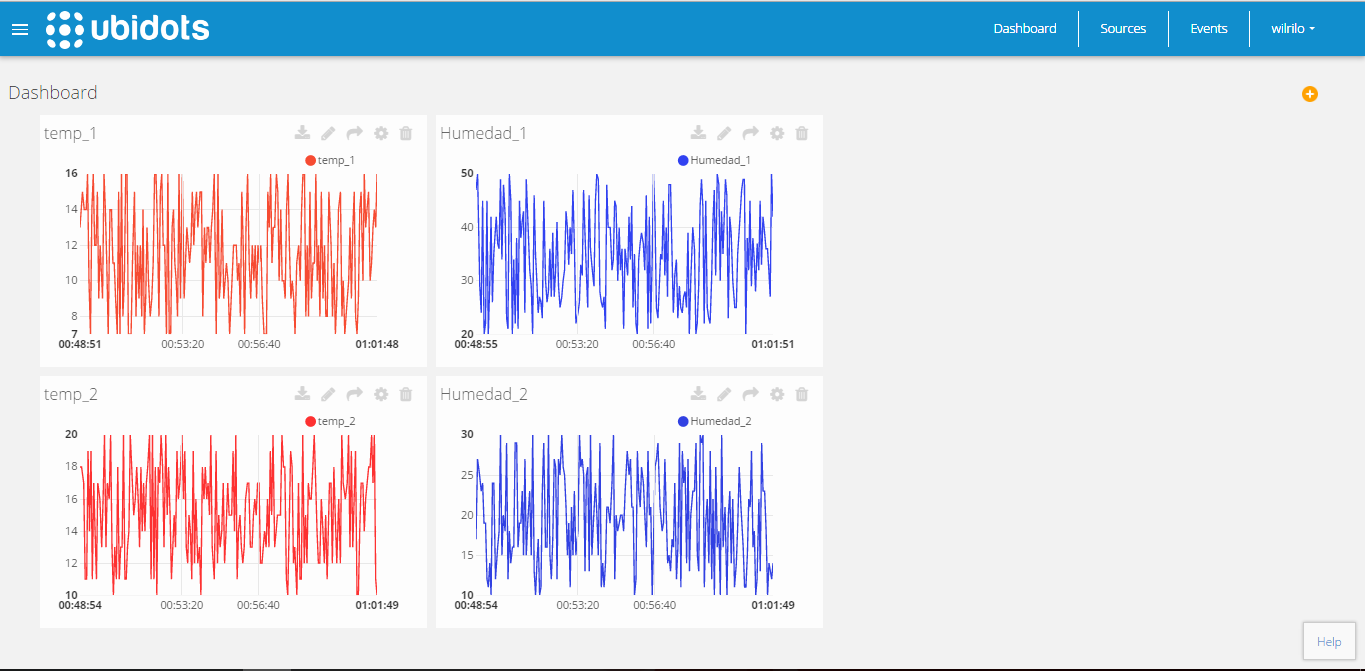
\includegraphics[scale=0.3]{ubi0}   % Scale se utiliza para cambiar el tamaño de la imagen
 		\caption{ Ubidots} 		
 	\end{figure}
\end{frame}

\begin{frame}
	\frametitle{Ubidots}
	
 	\begin{figure}[ht]
 		\centering
 		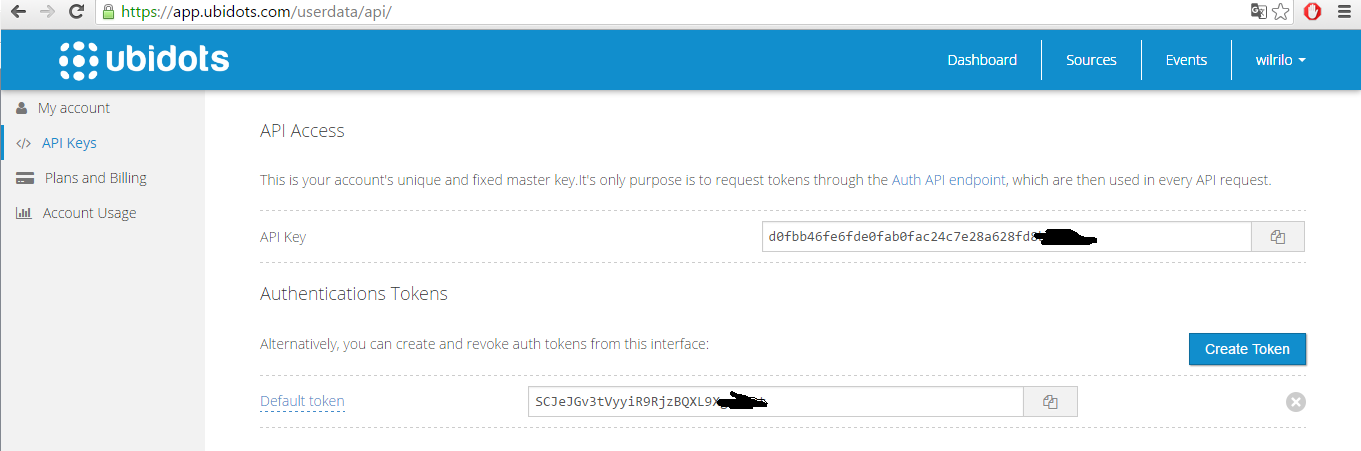
\includegraphics[scale=0.3]{ubi2}   % Scale se utiliza para cambiar el tamaño de la imagen
 		\caption{adquirir API y Token de Ubidots} 		
 	\end{figure}
\end{frame}

\begin{frame}
	\frametitle{Ubidots}
	
 	\begin{figure}[H]
 		\centering
 		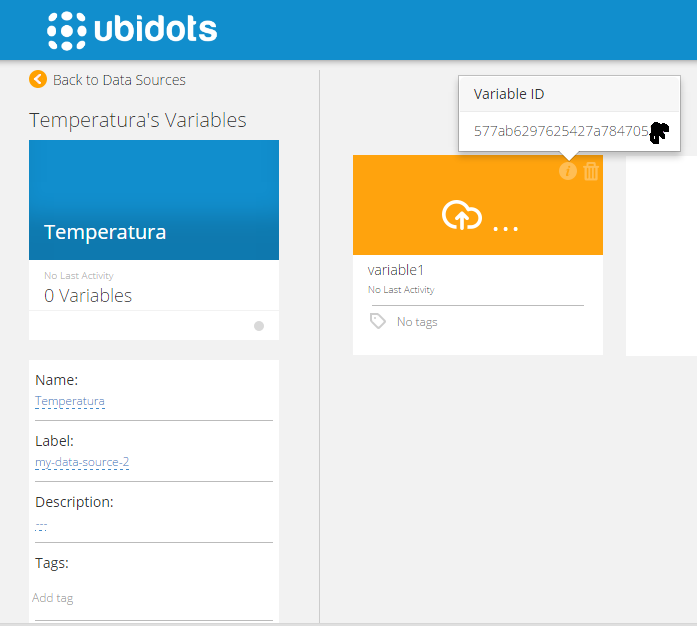
\includegraphics[scale=0.3]{ubi5}   % Scale se utiliza para cambiar el tamaño de la imagen
 		\caption{ID de las variables en Ubidots} 		
 	\end{figure}
\end{frame}



\begin{frame}
\frametitle{Programa en python}
 Crear la siguiente \href{https://github.com/wilrilo/repo_final_nube/tree/master/repo_final_nube/ProyectoF_Pi}{estructura de archivos}.
		\begin{figure}[ht] 
			\centering
			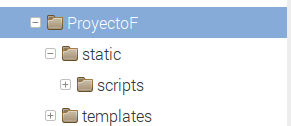
\includegraphics[scale=1]{estructura}   % Scale se utiliza para cambiar el tamaño de la imagen
			\caption{Estructura de archivos para trabajar en python}	
		\end{figure}
\end{frame}





\begin{frame}
\frametitle{\textbf{Codigo archivo \href{https://github.com/wilrilo/repo_final_nube/blob/master/repo_final_nube/ProyectoF_Pi/programa.py}{\texttt{programa.py}}:}}

En el archivo se importan las librerías:
\begin{itemize}
	\item Tornado
	\item timer
	\item random
	\item Ubidots
	
\end{itemize}

\end{frame}


\begin{frame}
\frametitle{API y ID's}
Se agregan la API y los ID's de Ubidots\\
\begin{center}
$api = ApiClient(token= 'SCJeJGv3tVyyiR9RjzBQXL9XgzCCxt')\\
humedad = api.get_variable("5763b2ab7625421ca1a7d82a")\\
temperatura = api.get_variable("5763ac2376254249a1fa9eba")$	
\end{center}


\end{frame}


\begin{frame}
\frametitle{configuración IPv6}
		\begin{figure}[H] 
			\centering
			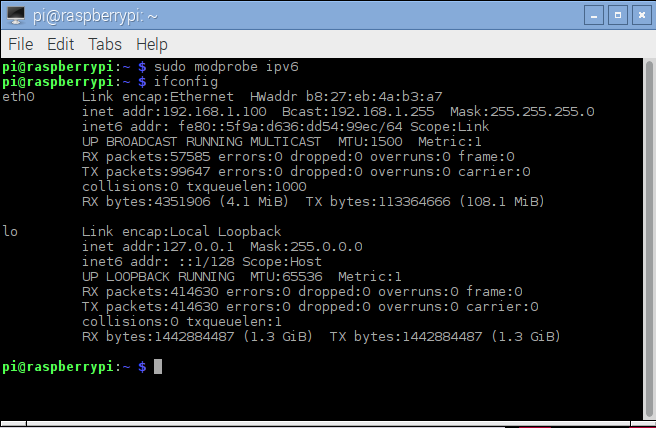
\includegraphics[scale=0.3]{ip6_1}   % Scale se utiliza para cambiar el tamaño de la imagen
			\caption{Configuración IPv6 raspberry pi}	
		\end{figure}
\end{frame}

\begin{frame}
	\frametitle{configuración IPv6}
		\begin{figure}[H] 
			\centering
			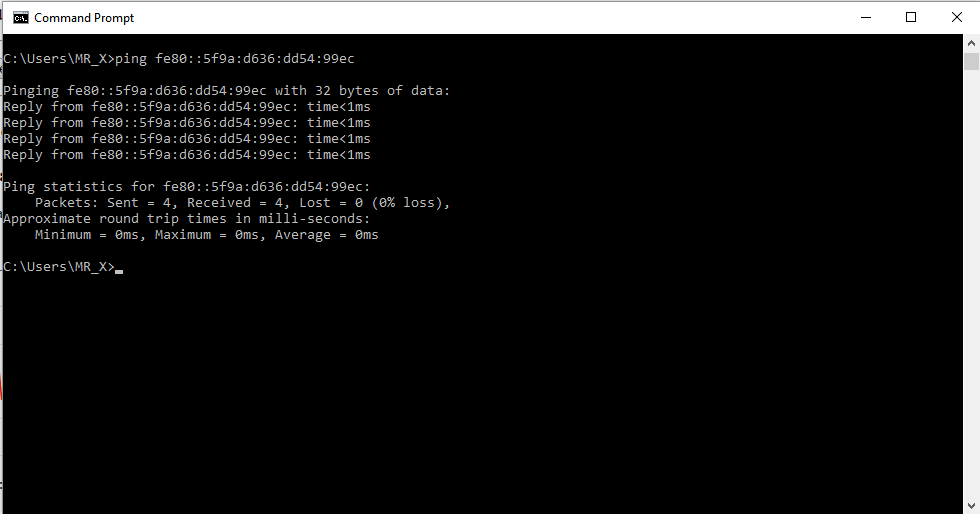
\includegraphics[scale=0.4]{ip6_2}  
			\caption{ping a la raspberry por protocolo IPv6 }	
		\end{figure}
\end{frame}

\begin{frame}
	\frametitle{configuración IPv6}
Abrimos un archivo llamado \href{https://github.com/wilrilo/repo_final_nube/blob/master/repo_final_nube/ProyectoF_Pi/static/scripts/raspberry.js}{raspberry.js} vamos a introducir la dirección IPv6 de la raspberry\\
\begin{center}
var ipDir = '//[fe80::5f9a:d636:dd54:99ec]:5000';	
\end{center}

\end{frame}


\begin{frame}
\frametitle{pagina HTML}
		\begin{figure}[H] 
			\centering
			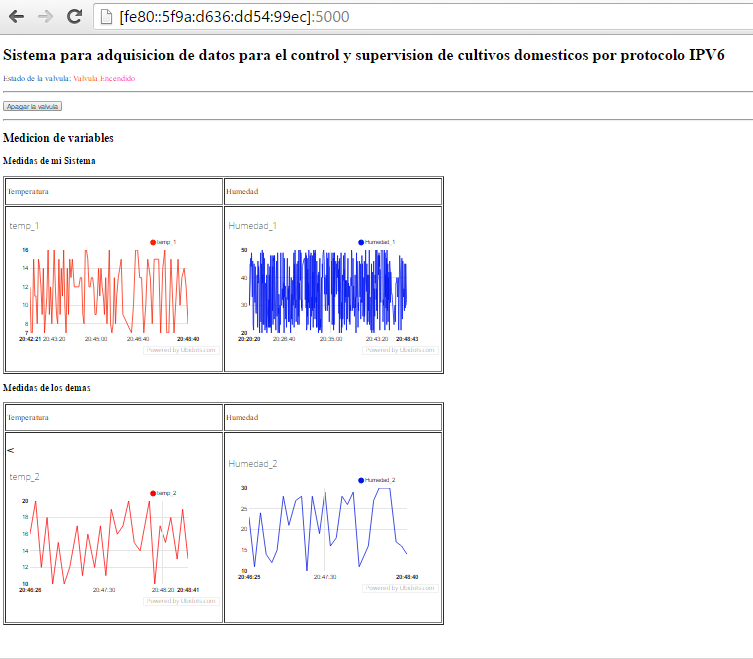
\includegraphics[scale=0.3]{html3}  
			\caption{pagina html}	
		\end{figure}
\end{frame}

\begin{frame}
	\frametitle{Ejecución del programa}
En la carpeta donde desarrollamos el proyecto en este caso \href{https://github.com/wilrilo/repo_final_nube/tree/master/repo_final_nube/ProyectoF_Pi}{\texttt{proyectoF\_Pi}} y escribimos el comando \texttt{python programa.py}:
\begin{figure}[H] 
	\centering
	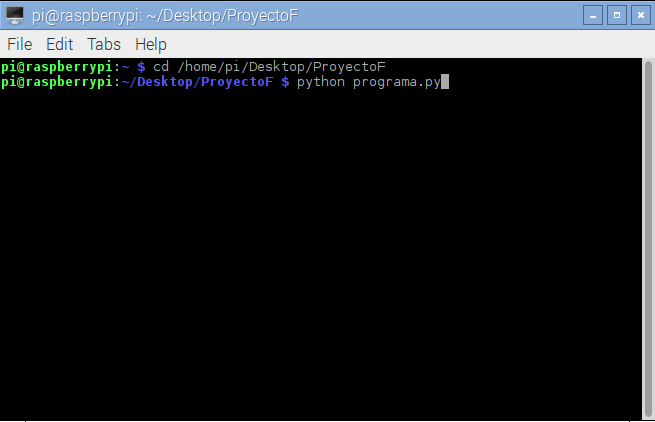
\includegraphics[scale=0.3]{eje1}  
	\caption{Comandos para ejecutar el programa}	
\end{figure}
\end{frame}

\begin{frame}[fragile]
	\frametitle{Análisis de los datos}
	se instalan y ejecutan los siguientes paquetes
\begin{knitrout}
\definecolor{shadecolor}{rgb}{0.969, 0.969, 0.969}\color{fgcolor}\begin{kframe}
\begin{alltt}
\hlkwd{library}\hlstd{(methods)}
\hlkwd{library}\hlstd{(jsonlite)}
\end{alltt}
\end{kframe}
\end{knitrout}
\end{frame}



\begin{frame}
	\frametitle{Análisis de los datos}
	Ubidots en R
\begin{knitrout}
\definecolor{shadecolor}{rgb}{0.969, 0.969, 0.969}\color{fgcolor}\begin{kframe}
\begin{alltt}
\hlstd{ubiURL}\hlkwb{<-}\hlstr{"http://things.ubidots.com/api/v1.6/variables/5763b2ab7625421ca1a7d82a/"}
\hlstd{ubiURL}\hlkwb{<-}\hlkwd{paste}\hlstd{(ubiURL,}\hlstr{"values/?token=SCJeJGv3tVyyiR9RjzBQXL9XgzCCxt"}\hlstd{,}\hlkwc{sep} \hlstd{=} \hlstr{""}\hlstd{)}
\end{alltt}
\end{kframe}
\end{knitrout}
\end{frame}

\begin{frame}
	\frametitle{Análisis de los datos}
	Ubidots en R
\begin{knitrout}
\definecolor{shadecolor}{rgb}{0.969, 0.969, 0.969}\color{fgcolor}\begin{kframe}
\begin{alltt}
\hlstd{ubidots} \hlkwb{<-} \hlkwd{fromJSON}\hlstd{(ubiURL)}
\hlstd{valores} \hlkwb{<-} \hlstd{ubidots}\hlopt{$}\hlstd{results}\hlopt{$}\hlstd{value}
\hlstd{tiempos} \hlkwb{<-} \hlstd{ubidots}\hlopt{$}\hlstd{results}\hlopt{$}\hlstd{time}
\hlstd{marcas} \hlkwb{<-} \hlstd{ubidots}\hlopt{$}\hlstd{results}\hlopt{$}\hlstd{created}
\end{alltt}
\end{kframe}
\end{knitrout}
\end{frame}

\begin{frame}[fragile]
	\frametitle{Análisis de los datos}
	Gráfica
	\begin{center}
\begin{knitrout}
\definecolor{shadecolor}{rgb}{0.969, 0.969, 0.969}\color{fgcolor}\begin{kframe}
\begin{alltt}
\hlkwd{plot}\hlstd{(tiempos,valores,}\hlstr{'l'}\hlstd{,}\hlkwc{col} \hlstd{=} \hlstr{"black"}\hlstd{,}\hlkwc{main} \hlstd{=} \hlstr{"Datos de humedad 1"}\hlstd{)}
\end{alltt}
\end{kframe}
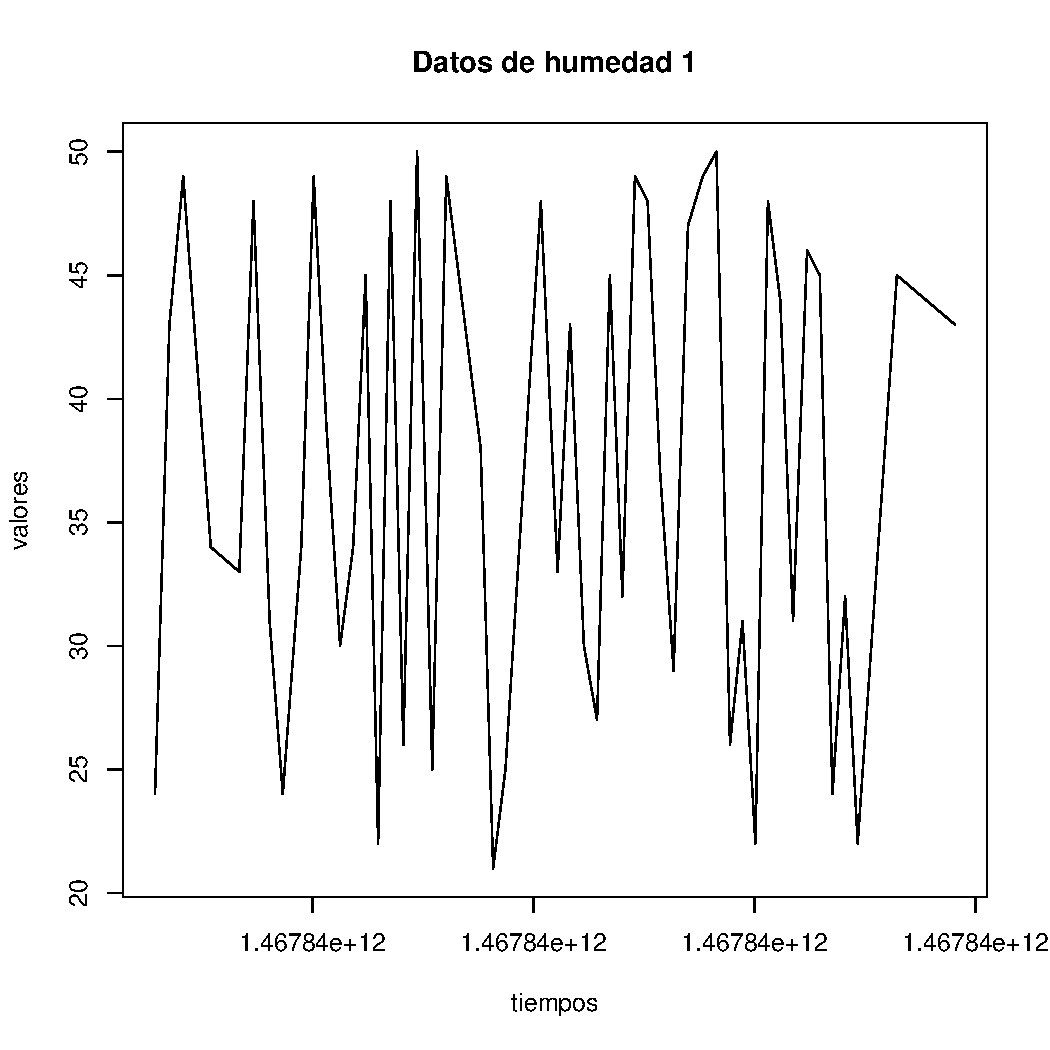
\includegraphics[width=2in]{figure/unnamed-chunk-4-1} 

\end{knitrout}
	 	
	\end{center}	
\end{frame}

\begin{frame}[fragile]
	\frametitle{Análisis de los datos}
	 estudio estadístico
\begin{knitrout}
\definecolor{shadecolor}{rgb}{0.969, 0.969, 0.969}\color{fgcolor}\begin{kframe}
\begin{alltt}
\hlkwd{mean}\hlstd{(valores)}
\end{alltt}
\begin{verbatim}
## [1] 36.94
\end{verbatim}
\begin{alltt}
\hlkwd{median}\hlstd{(valores)}
\end{alltt}
\begin{verbatim}
## [1] 35.5
\end{verbatim}
\begin{alltt}
\hlkwd{quantile}\hlstd{(valores)}
\end{alltt}
\begin{verbatim}
##    0%   25%   50%   75%  100% 
## 21.00 29.25 35.50 46.75 50.00
\end{verbatim}
\begin{alltt}
\hlkwd{var}\hlstd{(valores)}
\end{alltt}
\begin{verbatim}
## [1] 96.09837
\end{verbatim}
\end{kframe}
\end{knitrout}
\end{frame}

\begin{frame}[fragile]
	\frametitle{Análisis de los datos}
	estudio estadístico

\begin{knitrout}
\definecolor{shadecolor}{rgb}{0.969, 0.969, 0.969}\color{fgcolor}\begin{kframe}
\begin{alltt}
\hlcom{#humedad 1}
\hlstd{ubiURL}\hlkwb{<-}\hlstr{"http://things.ubidots.com/api/v1.6/variables/5763b2c87625421f2f017764/"}
\hlstd{ubiURL}\hlkwb{<-}\hlkwd{paste}\hlstd{(ubiURL,}\hlstr{"values/?token=SCJeJGv3tVyyiR9RjzBQXL9XgzCCxt"}\hlstd{,}\hlkwc{sep} \hlstd{=} \hlstr{""}\hlstd{)}
\hlstd{ubidots1} \hlkwb{<-} \hlkwd{fromJSON}\hlstd{(ubiURL)}
\hlstd{hum1} \hlkwb{<-} \hlstd{ubidots}\hlopt{$}\hlstd{results}\hlopt{$}\hlstd{value}
\hlstd{thume1} \hlkwb{<-} \hlstd{ubidots}\hlopt{$}\hlstd{results}\hlopt{$}\hlstd{time}
\hlcom{#humedad 2}
\hlstd{ubiURL}\hlkwb{<-}\hlstr{"http://things.ubidots.com/api/v1.6/variables/5763b2c87625421f2f017764/"}
\hlstd{ubiURL}\hlkwb{<-}\hlkwd{paste}\hlstd{(ubiURL,}\hlstr{"values/?token=SCJeJGv3tVyyiR9RjzBQXL9XgzCCxt"}\hlstd{,}\hlkwc{sep} \hlstd{=} \hlstr{""}\hlstd{)}
\hlstd{ubidots2} \hlkwb{<-} \hlkwd{fromJSON}\hlstd{(ubiURL)}
\hlstd{hum2} \hlkwb{<-} \hlstd{ubidots}\hlopt{$}\hlstd{results}\hlopt{$}\hlstd{value}
\hlstd{thume2} \hlkwb{<-} \hlstd{ubidots}\hlopt{$}\hlstd{results}\hlopt{$}\hlstd{time}

\hlcom{#temperatura 1}
\hlstd{ubiURL}\hlkwb{<-}\hlstr{"http://things.ubidots.com/api/v1.6/variables/5763ac2376254249a1fa9eba/"}
\hlstd{ubiURL}\hlkwb{<-}\hlkwd{paste}\hlstd{(ubiURL,}\hlstr{"values/?token=SCJeJGv3tVyyiR9RjzBQXL9XgzCCxt"}\hlstd{,}\hlkwc{sep} \hlstd{=} \hlstr{""}\hlstd{)}
\hlstd{ubidots1} \hlkwb{<-} \hlkwd{fromJSON}\hlstd{(ubiURL)}
\hlstd{tem1} \hlkwb{<-} \hlstd{ubidots}\hlopt{$}\hlstd{results}\hlopt{$}\hlstd{value}
\hlstd{ttem1} \hlkwb{<-} \hlstd{ubidots}\hlopt{$}\hlstd{results}\hlopt{$}\hlstd{time}
\hlcom{#temperatura 2}
\hlstd{ubiURL}\hlkwb{<-}\hlstr{"http://things.ubidots.com/api/v1.6/variables/5763b35276254225fcaaa266/"}
\hlstd{ubiURL}\hlkwb{<-}\hlkwd{paste}\hlstd{(ubiURL,}\hlstr{"values/?token=SCJeJGv3tVyyiR9RjzBQXL9XgzCCxt"}\hlstd{,}\hlkwc{sep} \hlstd{=} \hlstr{""}\hlstd{)}
\hlstd{ubidots2} \hlkwb{<-} \hlkwd{fromJSON}\hlstd{(ubiURL)}
\hlstd{tem2} \hlkwb{<-} \hlstd{ubidots}\hlopt{$}\hlstd{results}\hlopt{$}\hlstd{value}
\hlstd{ttem2} \hlkwb{<-} \hlstd{ubidots}\hlopt{$}\hlstd{results}\hlopt{$}\hlstd{time}
\end{alltt}
\end{kframe}
\end{knitrout}
	
\end{frame}

\begin{frame}[fragile]
	\frametitle{Análisis de los datos}
	estudio estadístico
	\begin{center}
\begin{knitrout}
\definecolor{shadecolor}{rgb}{0.969, 0.969, 0.969}\color{fgcolor}\begin{kframe}
\begin{alltt}
\hlkwd{par}\hlstd{(}\hlkwc{mfrow}\hlstd{=}\hlkwd{c}\hlstd{(}\hlnum{2}\hlstd{,}\hlnum{2}\hlstd{))}
\hlkwd{plot}\hlstd{(thume1,hum1,}\hlstr{'l'}\hlstd{,}\hlkwc{col} \hlstd{=} \hlstr{"blue"}\hlstd{,}\hlkwc{main} \hlstd{=} \hlstr{"Datos de humedad 1"}\hlstd{)}
\hlkwd{plot}\hlstd{(thume2,hum2,}\hlstr{'l'}\hlstd{,}\hlkwc{col} \hlstd{=} \hlstr{"blue"}\hlstd{,}\hlkwc{main} \hlstd{=} \hlstr{"Datos de humedad 2"}\hlstd{)}
\hlkwd{plot}\hlstd{(ttem1,tem1,}\hlstr{'l'}\hlstd{,}\hlkwc{col} \hlstd{=} \hlstr{"red"}\hlstd{,}\hlkwc{main} \hlstd{=} \hlstr{"Datos de Temperatura 1"}\hlstd{)}
\hlkwd{plot}\hlstd{(ttem2,tem2,}\hlstr{'l'}\hlstd{,}\hlkwc{col} \hlstd{=} \hlstr{"red"}\hlstd{,}\hlkwc{main} \hlstd{=} \hlstr{"Datos de Temperatura 2"}\hlstd{)}
\end{alltt}
\end{kframe}
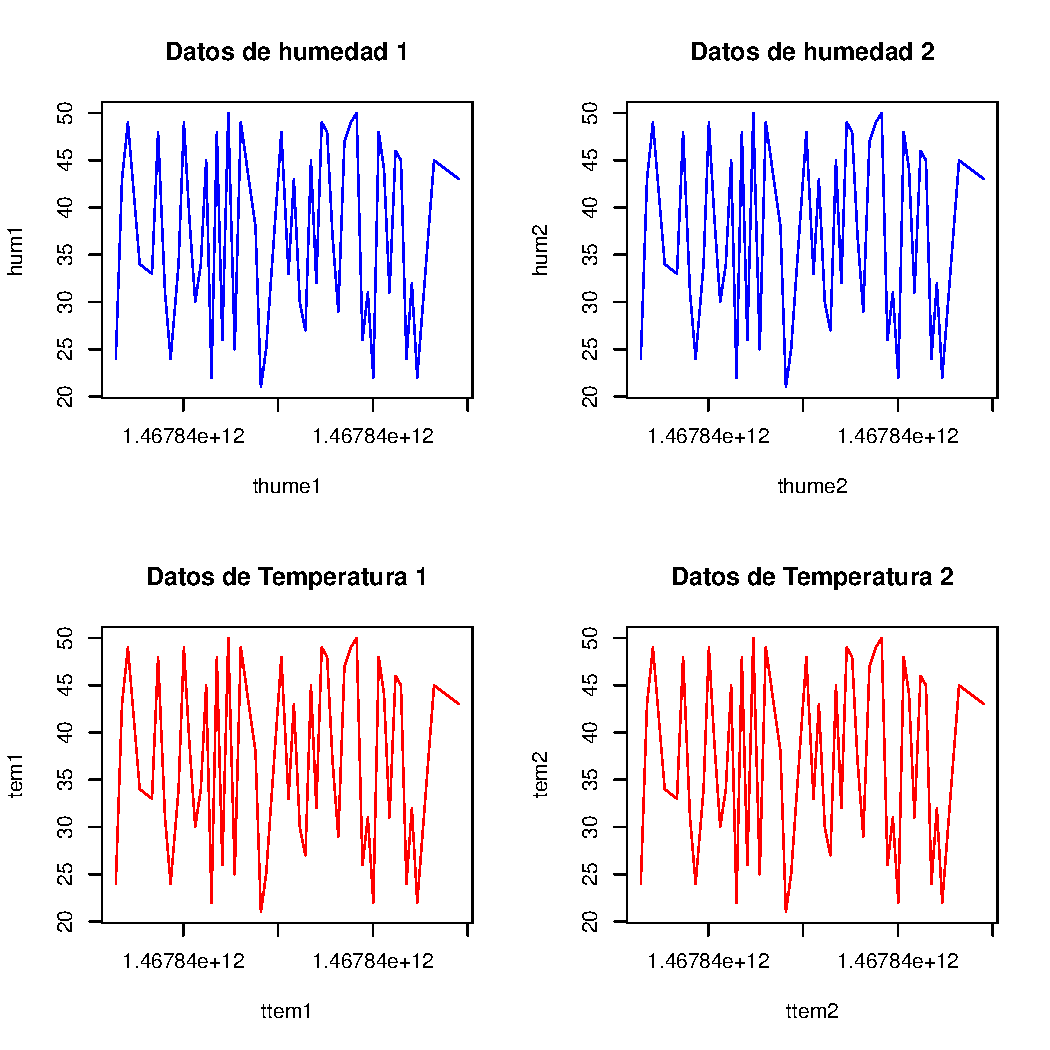
\includegraphics[width=2in]{figure/unnamed-chunk-8-1} 

\end{knitrout}
	\end{center}
	
\end{frame}


\begin{frame}
\frametitle{Bibliografía}
	\begin{enumerate}
		\item  \href{http://silicio.mx/sensor-de-humedad-grove}{características sensor de humedad}
		\href{http://rita.udistrital.edu.co/index.php/servicios/servicios-internos/direccionamiento-ipv6-y-dns}{soporte rita IPv6}
		\item \href{	http://articulo.mercadolibre.com.mx/MLM-550669563-arduino-ethernet-shield-generico-atmel-robotica-_JMredirectedFromParent}{imagen arduino}
		\item \href{http://www.reflexiona.biz/shop/temperatura/559--sensor-de-temperatura-lm335a.html}{imagen sensor de temperatura}
		\item \href{http://www.atomsindustries.com/ASD1055}{imagen rasberry pi}
		
		\item \href{https://www.minagricultura.gov.co/}{ministerioagricultura}
		
		\item \href{http://ambientebogota.gov.co/techos-verdes-y-jardines-verticalessthash.tSdqSq1s.dpuf
		}{http://ambientebogota.gov.co/techos-verdes-y-jardines-verticalessthash.tSdqSq1s.dpuf [fecha de consulta: 22 de agosto de 2015]
	}
	
	\item \href{http://ambientebogota.gov.co/web/una-piel-natural-para-bogota//consulta-la-guia-tecnica-de-techos-}{http://ambientebogota.gov.co/web/una-piel-natural-para-bogota//consulta-la-guia-tecnica-de-techos-[fecha de consulta: 22 de agosto de 2015]}
	
	\item \href{http://www.eltiempo.com/colombia/cali/proyecto-vive-digital-llega-a-escuelas-de-narino/14681459}{http://www.eltiempo.com/colombia/cali/proyecto-vive-digital-llega-a-escuelas-de-narino/14681459[fecha de consulta: 22 de agosto de 2015]}
	
	\item \href{http://weblog.aklmedia.nl/tag/raspberry-pi/}{http://weblog.aklmedia.nl/tag/raspberry-pi/}
	
	
	%  
	
	%[13] 	%
	%
	%
	%[14]
	%verdes-para-bogota . 
	
	% granjasdigi
	%[15] http://www.eltiempo.com/colombia/cali/proyecto-vive-digital-llega-a-escuelas-de-narino/14681459 .
	%
	%[fecha de consulta: 22 de agosto de 2015]
	
	%% http://weblog.aklmedia.nl/tag/raspberry-pi/
\end{enumerate}
\end{frame}


\end{document}
